\documentclass[border=3pt,tikz]{standalone}
\usepackage{amsmath}
\usetikzlibrary{arrows.meta}
\usetikzlibrary{calc}
\usetikzlibrary{hobby}

\begin{document}
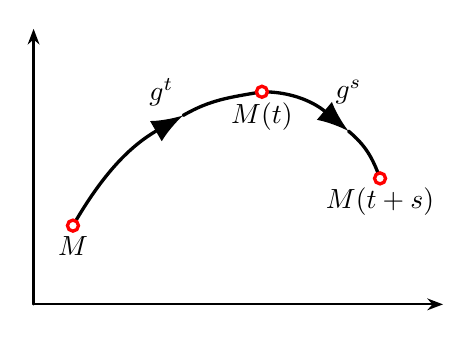
\begin{tikzpicture}[line cap=round, scale = 1]
    \coordinate (A) at (0.3, 0.5);
    \coordinate (B) at (1.7, 1.9);
    \coordinate (C) at (2.7, 2.2);
    \coordinate (D) at (3.8, 1.7);
    \coordinate (E) at (4.2, 1.1);

    \draw[thick, -{Stealth[length=2mm]}] (-0.2, -0.5) -- (5, -0.5);
    \draw[thick, -{Stealth[length=2mm]}] (-0.2, -0.5) -- (-0.2, 3);
    \draw[very thick, -{LaTeX[length=4mm]}] (A) to[out=60, in=210](B) ;
    \draw[very thick,] (B) to[out=30, in=190](C) ;
    \draw[very thick,-{LaTeX[length=4mm]}] (C) to[out=0, in=140](D) ;
     \draw[very thick,] (D) to[out=320, in=110](E) ;
    
    \draw[red, fill=white, very thick] (A) circle (0.07) node[below, black] {$M$};
    \node[above left] at (B) {$g^t$};
    \draw[red, fill=white, very thick] (C) circle (0.07) node [below, black] {$M(t)$};
    \node [yshift=0.5cm] at (D) {$g^s$};
    \draw[red, fill=white, very thick] (E) circle (0.07);
    \node[below] at (E) {$M(t+s)$};
    \end{tikzpicture}
\end{document}